\documentclass[professionalfonts]{beamer}

\usepackage[T1]{fontenc}
\usepackage[brazil]{babel}
\usepackage[utf8]{inputenc}

\usepackage{booktabs,multirow,longtable}
\usepackage{amsmath,amsfonts,amssymb}
\usepackage{bm}

\usepackage{subfig}
\usepackage[round]{natbib}

% Coisas adicionadas para ativar os overlays co Tikz
\usepackage{tikz}
\usetikzlibrary{arrows,shapes}

% Choose the Inf theme
\usetheme{Inf}

\usepackage[linesnumbered,ruled,vlined]{algorithm2e}
\SetArgSty{textnormal}
\DontPrintSemicolon

% Define the title with \title[short title]{long title}
% Short title is optional
\title[GRASP+BL para Flowshop]{Metaheurística GRASP com refinamento por busca local para o Flowshop Permutacional}

% Optional subtitle
\subtitle{Otimização Combinatória --- INF05010}

\date{2019/2}

% Author information
\author{Alberto F. K. Neto}
\institute{CUSTOM LAST PAGE, CHECK BELOW}

% Disable pdflatex warnings about tiny bad boxes
% Show a indicator of badboxes
% \hfuzz=2pt
% \overfullrule=50pt

\begin{document}

% Command to create title page
\InfTitlePage%

\begin{frame}
   \frametitle{Agenda}
   \tableofcontents
\end{frame}

\section{Introdução}

\begin{frame}
   \frametitle{Sobre o trabalho desenvolvido}

   \textbf{Flowshop permutacional}
   \begin{itemize}
      \item Tópico de pesquisa recorrente em Otimização Combinatória
      \item Grande interesse acadêmico e aplicado
      \item Fácil obter soluções factíveis
      \item Difícil de provar uma solução ótima
   \end{itemize}

   \medskip
   \textbf{Sobre o trabalho desenvolvido}
   \begin{itemize}
      \item Formulação inteira mista de \cite{tseng2004-flowshop-models}
      \item Solução construtiva com GRASP
      \item Melhoramento por Busca Local
      \item Comparação de desempenho
   \end{itemize}
\end{frame}

\section{Definição do Problema}

\begin{frame}
   \frametitle{Flowshop Permutacional}

   \textbf{Dados do problema}
   \begin{itemize}
      \item $N$ tarefas
      \item $M$ máquinas
      \item $T_{ri} \geqslant 0$ tempo de processamento ($1 \leqslant i \leqslant N$ 
         ; $1 \leqslant r \leqslant M$)
   \end{itemize}

   \medskip
   \textbf{Objetivo:} Minimizar tempo de processamento final da máquina $M$

   \medskip
   \textbf{Solução:} Ordem de execução das tarefas

   \medskip
   \textbf{Restrições}
   \begin{itemize}
      \item Mesma ordem em todas as máquinas
      \item Processamento completo na máquina anterior antes de prosseguir 
   \end{itemize}
\end{frame}

\begin{frame}
   \frametitle{Flowshop Permutacional}

   \medskip
   \textbf{Exemplo de instância}
   \begin{itemize}
      \item $N = 5$
      \item $M = 4$
      \item Solução de custo $z = 35$
   \end{itemize}

   \begin{figure}
      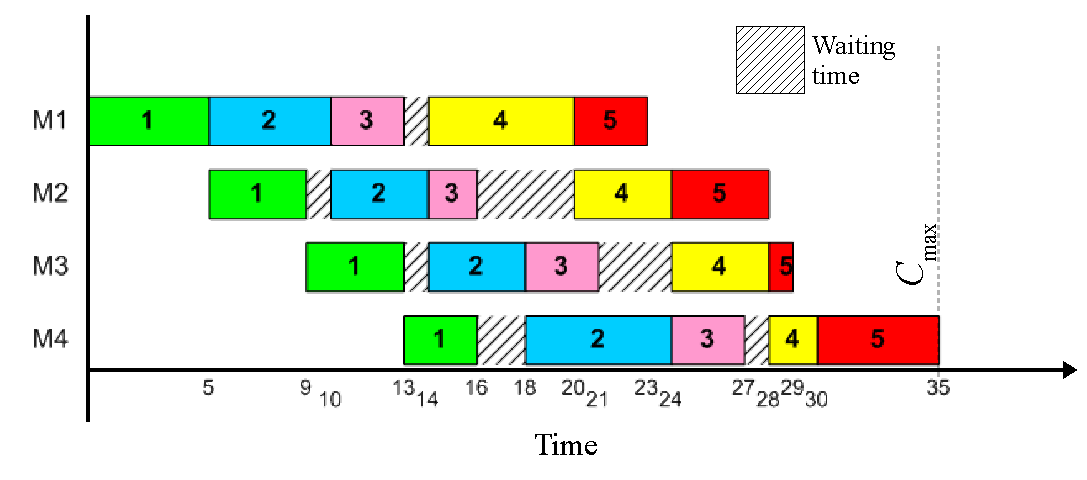
\includegraphics[width=0.9\textwidth]{img/pfsp-my}
   \end{figure}
\end{frame}

\begin{frame}
   \frametitle{Formulação matemática}

   \textbf{Variáveis de decisão}
   \begin{itemize}
      \item \textcolor{red}{$D_{ik} \in \{0,1\}$:} Indica se a tarefa $i$ é
         processada antes da tarefa $k$, para $1 \leqslant i < k \leqslant N$
      \item \textcolor{blue}{$C_{ri} \geqslant 0$:} Tempo em que a tarefa $i$
         termina de ser processada na máquina $r$, para $1 \leqslant i 
         \leqslant N$ e $1 \leqslant r \leqslant M$
      \item \textcolor{blue}{$C_\mathrm{max}$:} Tempo de processamento final da
         última máquina
   \end{itemize}

   \medskip
   \textbf{Parâmetros}
   \begin{itemize}
      \item $T_{ri} \geqslant 0$: Tempos de processamento
      \item $P$: Valor suficientemente grande
   \end{itemize}
\end{frame}

\begin{frame}
   \frametitle{Formulação matemática}

   \begin{align}
      \text{Minimize } C_\mathrm{max} \label{pfsp:obj}
   \end{align}
   Sujeito a:
   \begin{align}
      & C_{1i} \geqslant T_{1i} & & 1 \leqslant i \leqslant N \label{pfsp:complM0} \\
      & C_{ri} - C_{r-1,i} \geqslant T_{ri} & & 2 \leqslant r \leqslant M, 
         1 \leqslant i \leqslant N \label{pfsp:complM} \\
      & C_{ri} - C_{rk} + PD_{ik} \geqslant T_{ri} & & 1 \leqslant r \leqslant M, 
         1 \leqslant i < k \leqslant N \label{pfsp:jobSeqA}\\
      & C_{ri} - C_{rk} + PD_{ik} \leqslant P - T_{rk} & & 1 \leqslant r \leqslant M, 
         1 \leqslant i < k \leqslant N \label{pfsp:jobSeqB} \\
      & C_\mathrm{max} \geqslant C_{Mi} & & 1 \leqslant i \leqslant N \label{pfsp:makespan} \\
      & C_{ri} \geqslant 0 & & 1 \leqslant r \leqslant M, 1 \leqslant i \leqslant N \label{pfsp:Cdom}\\
      & D_{ik} \in \{0,1\} & & 1 \leqslant i < k \leqslant N \label{pfsp:Ddom}
   \end{align}
\end{frame}

\section{Método heurístico de resolução}

\begin{frame}
   \frametitle{Construtivo com GRASP}

   \textbf{Sobre o GRASP}
   \begin{itemize}
      \item Proposto por \cite{feo1994-grasp}
      \item Método construtivo guloso randomizado
      \item Parâmetro de randomização $\alpha \in [0,1]$
   \end{itemize}

   \medskip
   \textbf{Detalhes de implementação}
   \begin{itemize}
      \item Lista com ordem de execução
      \item Tempos em estrutura de dados 2D 
      \item Randomização controlada com sementes
   \end{itemize}
\end{frame}

\begin{frame}
   \frametitle{Construtivo com GRASP}

   \begin{algorithm}[H]
      \footnotesize
      \SetKwFunction{proc}{GRASP}
      \SetKwProg{myproc}{Procedure}{}{}
      \myproc{\proc{$N$, $M$, $T$, $\alpha$}}{
         $\mathit{pend} \gets$ lista com valores $1, 2, \dots, N$ \;
         $s \gets $ lista vazia; $z \gets 0$ \;
         \While{$\mathit{pend}$ não está vazia}{
            $\mathit{RCL} \gets $ lista vazia \;
            \For{$j \in \mathit{pend}$}{
               $\bar{z}_j \gets$ custo da solução parcial $s$ com adição da tarefa $j$ \; 
               adicione a tupla $(j, \bar{z}_j)$ em $\mathit{RCL}$ \;
            }
            ordene $\mathit{RCL}$ em ordem não crescente de $\bar{z}$ \;
            $\mathit{tam} \gets$ tamanho da lista $\mathit{RCL}$ \;
            $\mathit{tp} \gets$ escolhe aleatoriamente um índice 
               de $[1, \max\{1, \alpha \cdot \mathit{tam}\} ]$ \;
            atualize a solução $s$ e custo $z$ com os dados da tupla $\mathit{RCL}_\mathit{tp}$ \;
            remova a tarefa referente a $\mathit{tp}$ de $\mathit{pend}$ \;
         }
      }
      \Return{$s$}
      \caption{Construção de solução inicial com GRASP.}
      \label{algo:GRASP}
   \end{algorithm}
\end{frame}

\begin{frame}
   \frametitle{Busca Local}

   \textbf{Estratégia randomizada}
   \begin{itemize}
      \item Troca de duas tarefas aleatórias
      \item Sempre aceita uma melhora
      \item Busca local rápida e iterada
   \end{itemize}

   \begin{algorithm}[H]
      \footnotesize
      \SetKwFunction{proc}{Swap2LS}
      \SetKwProg{myproc}{Procedure}{}{}
      \myproc{\proc{$s^*$, numVezes}}{
         $z^* \gets$ custo da solução atual\;
         \For {$i \gets 1$ até $numVezes$} {
            selecione tarefas $j_1 \neq j_2$ aleatoriamente, com distribuição uniforme \;
            $\bar{s} \gets$ troque a ordem de processamento de $j_1 \leftrightarrow j_2$ em $s^*$ \;
            $\bar{z} \gets$ avalie o custo da solução $\bar{s}$ \;
            \If {$\bar{z} < z^*$} {
               $s^* \gets \bar{s}$ \;
               $z^* \gets \bar{z}$ \;
            }
         }
      }
      \Return $s*$
      \caption{Algoritmo de Busca Local.}
      \label{algo:LS}
   \end{algorithm}

\end{frame}

\begin{frame}
   \frametitle{Heurística completa}

   \begin{algorithm}[H]
      \footnotesize
      \SetKwFunction{proc}{GRASP\_LS}
      \SetKwProg{myproc}{Procedure}{}{}
      \myproc{\proc{$N$, $M$, $T$, $\alpha$}}{
         $s \gets$ \texttt{GRASP}($N$, $M$, $T$, $\alpha$) \;
         \For{$\mathit{iter} \gets 1$ até $\textit{MAX\_ITER}$ } {
            \texttt{Swap2LS}($s$, $\lceil N/100 \rceil$) \;
            \texttt{Swap2LS}($s$, $\lceil \mathit{iter}/1000 \rceil$) \;
            \texttt{Swap2LS}($s$, \texttt{randomInt}(1,N)) \;
         }
      }
      \Return $s$
      \caption{Heurística GRASP com Busca Local.}
      \label{algo:full}
   \end{algorithm}

\end{frame}

\section{Experimentos computacionais}

\begin{frame}
   \frametitle{Ambiente de testes}
   
   \textbf{Hardware e software}
   \begin{itemize}
      \item Intel 3612QM @ 2.10GHz, RAM 8GB
      \item GLPK 4.65
      \item Heurística em Python 3.7.4
      \item Arch Linux (kernel linux-5.3.8)
   \end{itemize}

   \medskip
   \textbf{Experimentos realizados}
   \begin{itemize}
      \item Solver por até 1h
      \item Heurística por até 2140 iterações
      \item $\alpha \in \{0, 0.2, 0.4, 0.6, 0.8, 1.0\}$
      \item 10 replicações por (instância,$\alpha$)
   \end{itemize}

\end{frame}

\begin{frame}
   \frametitle{Resultados com GLPK}

   \begin{table}[H]
      \centering
      \scriptsize
      \begin{tabular}{lrrrr}
         \toprule
         Instância & BKS & Valor relaxação & Obj. solução inteira & GAP$_\mathrm{BKS}$ (\%) \\
         \midrule
         VFR10\_15\_1 & 1307 & 880,0 & 1307\footnote[frame]{Após 1244,7 segundos de
         processamento.} & \phantom{0}0,0\\
         VFR10\_10\_3 & 1592 & 687,0 & 1873 & 56,9\\
         VFR\_20\_20\_1 & 2270 & 1391,0 & 2573 & 42,6\\
         VFR60\_5\_10 & 3663 & 382,0 & 3878 & 89,3\\
         VFR100\_60\_1 & 9395  &  TL & -- & $\infty$\\
         VFR500\_40\_1 & 28548 &  TL & -- & $\infty$\\
         VFR500\_60\_3 & 31125 &  TL & -- & $\infty$\\
         VFR600\_20\_1 & 31433 &  TL & -- & $\infty$\\
         VFR700\_20\_10 & 36417 & TL & -- & $\infty$\\ 
         \bottomrule
      \end{tabular}
      \caption{Resultado obtido por meio do GLPK.}
      \label{table:results-glpk}
   \end{table}

\end{frame}

\begin{frame}
   \frametitle{Resultados com heurística}

   \begin{table}[H]
      \centering
      \fontsize{5}{7}\selectfont
      \begin{tabular}{lrcccccc}
         \toprule
         \multirow{2}[2]{*}{Instância} & \multirow{2}[2]{*}{BKS} & \multicolumn{2}{c}{Sol. GRASP} & 
            \multicolumn{3}{c}{Sol. GRASP+BL}\\ \cmidrule(r){3-4} \cmidrule{5-7}
         & & F.O. & Desvio (\%) & F.O. & Desvio (\%) & Tempo (seg.)\\
         \midrule
         VFR10\_15\_1 & 1307 & $1424 \pm 0$ & 8,95 & $1339,6 \pm 18,319$ & 2,49 & $1,5$ \\ 
         VFR20\_10\_3 & 1592 & $2017 \pm 0$ & 26,70 & $1687,5 \pm 29,304$ & 6 & $2,1$ \\ 
         VFR20\_20\_1 & 2270 & $2715 \pm 0$ & 19,60 & $2360,1 \pm 33,478$ & 3,97 & $3,9$ \\ 
         VFR60\_5\_10 & 3663 & $3849 \pm 0$ & 5,08 & $3668,4 \pm 7,291$ & 0,15 & $3,2$ \\ 
         VFR60\_10\_3 & 3423 & $4357 \pm 0$ & 27,29 & $3632,6 \pm 62,45$ & 6,12 &
         $6,0$ \\ 
         VFR100\_60\_1 & 9395  & $11247 \pm 0$ & 19,71 & $10008,8 \pm 47,123$ & 6,53 & $57,7$ \\ 
         VFR500\_40\_1 & 28548 & $33119 \pm 0$ & 16,01 & $30640,6 \pm 67,832$ & 7,33 & $200,4$ \\ 
         VFR500\_60\_3 & 31125 & $36930 \pm 0$ & 18,65 & $33539,6 \pm 106,966$ & 7,76 & $298,5$ \\ 
         VFR600\_20\_1 & 31433 & $35473 \pm 0$ & 12,85 & $32904,4 \pm 69,306$ & 4,68 & $118,4$ \\ 
         VFR700\_20\_10 & 36417 & $40916 \pm 0$ & 12,35 & $37857,4 \pm 114,996$ & 3,96 & $140,6$ \\ 
         \bottomrule
      \end{tabular}
      \caption{Resultados médios da heurística para $\bm{\alpha = 0}$.} 
      \label{table:results-heur-short}
   \end{table}

\end{frame}

\begin{frame}
   \frametitle{Efeito da busca local}

   \begin{figure}
      \centering
      \only<1>{
         \subfloat{
            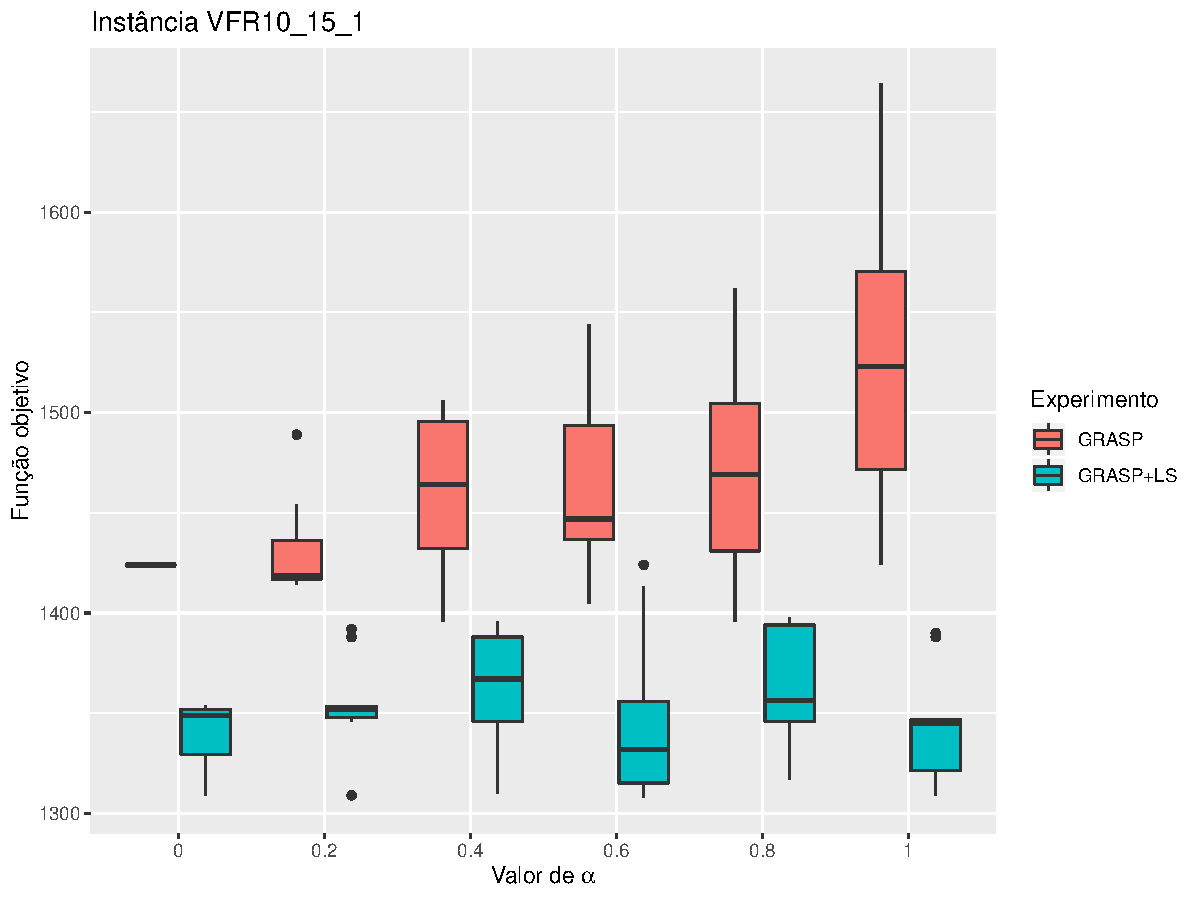
\includegraphics[width=0.48\textwidth]{../resultados/boxplot-VFR10_15_1.pdf}
         }
         \subfloat{
            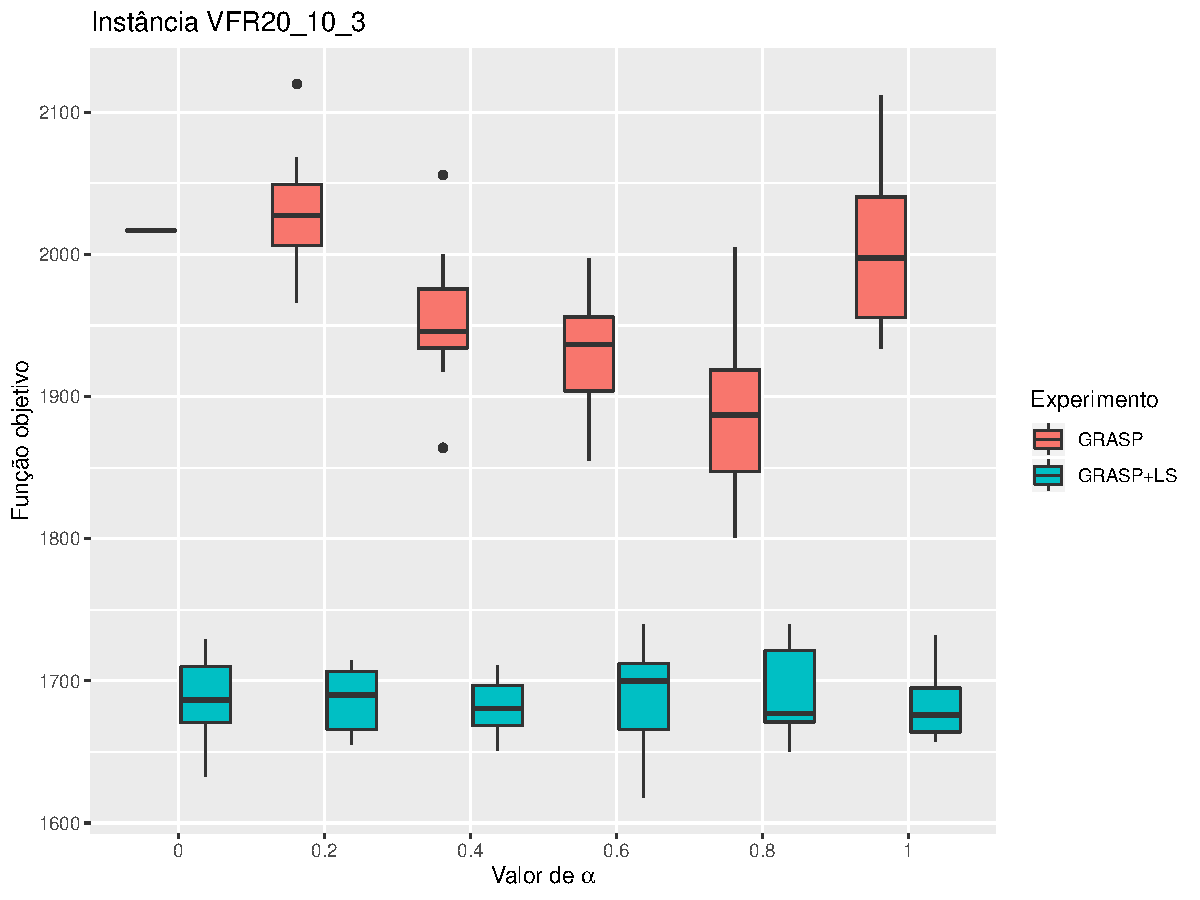
\includegraphics[width=0.48\textwidth]{../resultados/boxplot-VFR20_10_3.pdf}
         }\\
      }
      \only<2>{
         \subfloat{
            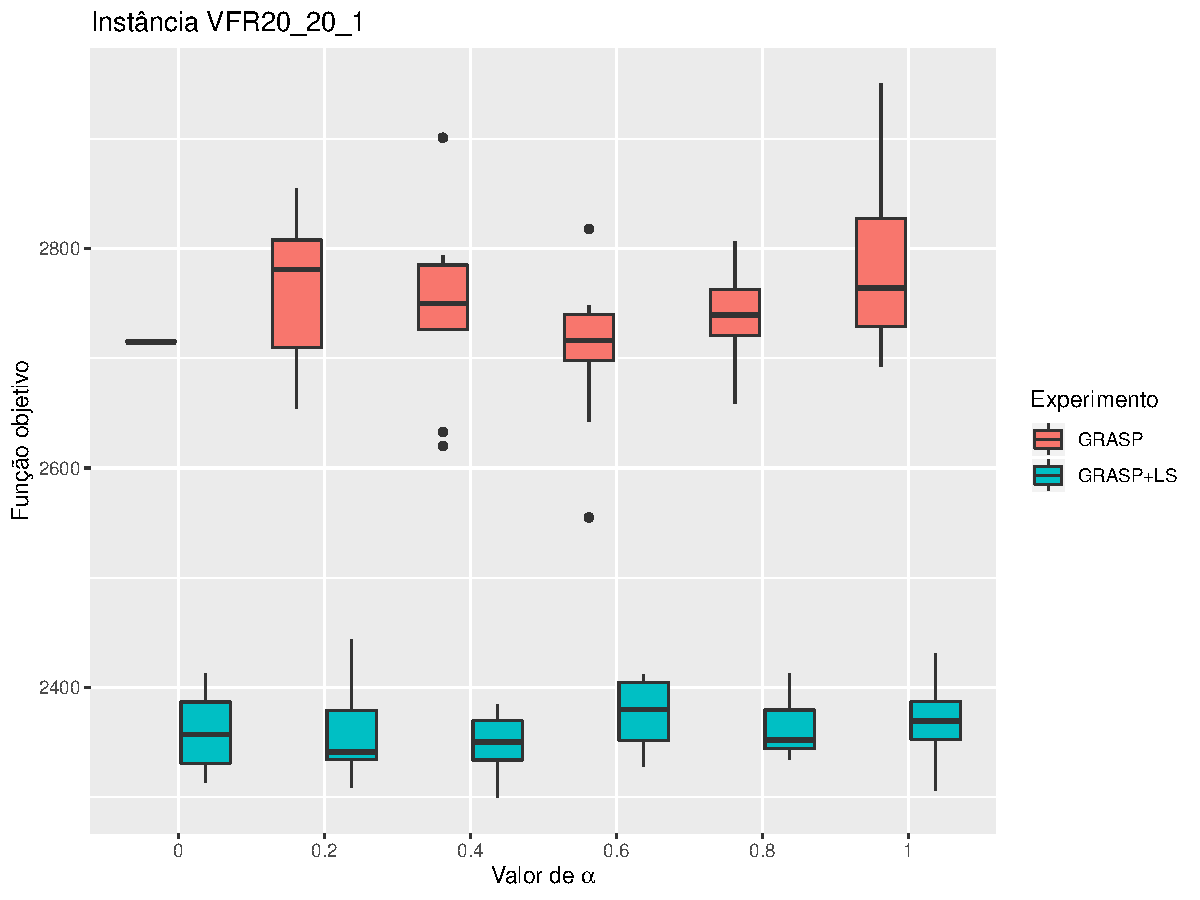
\includegraphics[width=0.48\textwidth]{../resultados/boxplot-VFR20_20_1.pdf}
         }
         \subfloat{
            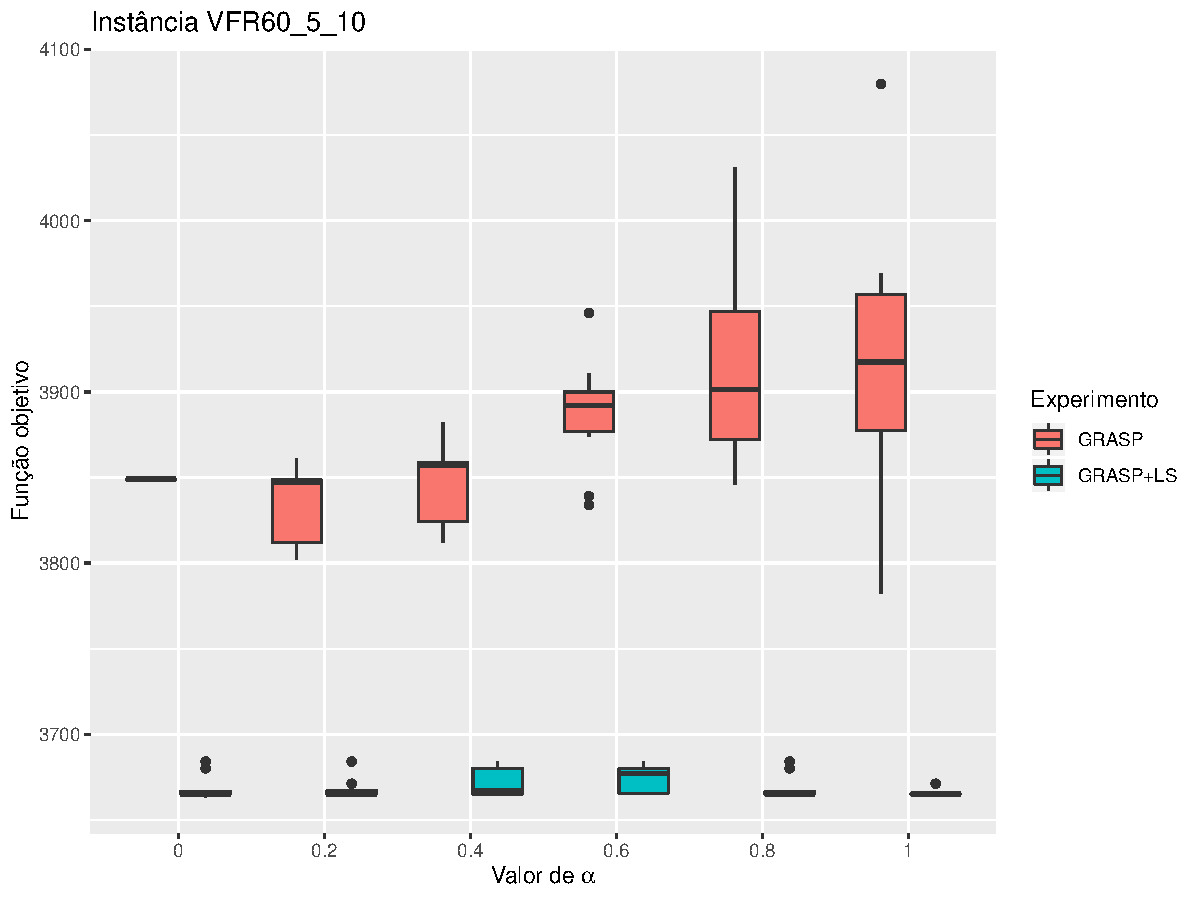
\includegraphics[width=0.48\textwidth]{../resultados/boxplot-VFR60_5_10.pdf}
         }\\
      }
      \only<3>{
         \subfloat{
            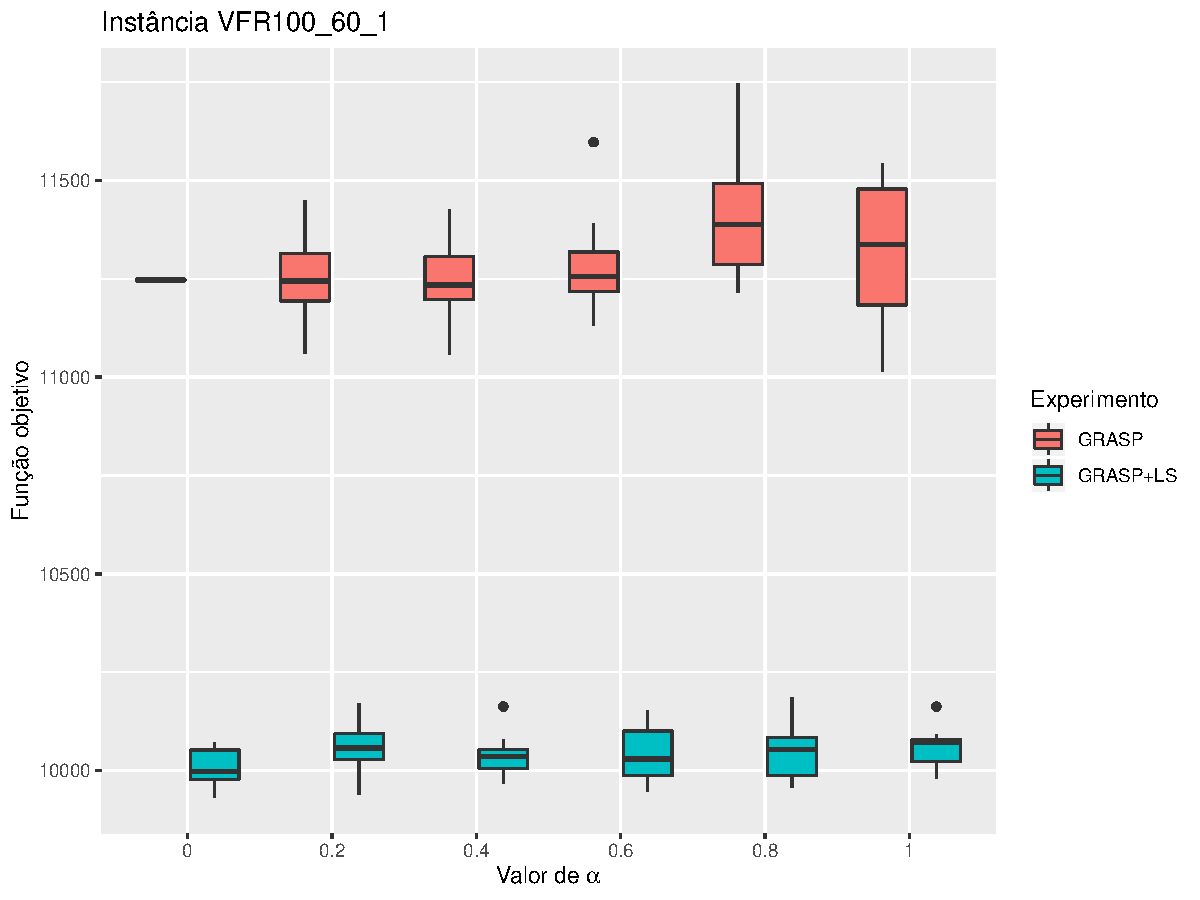
\includegraphics[width=0.48\textwidth]{../resultados/boxplot-VFR100_60_1.pdf}
         }
         \subfloat{
            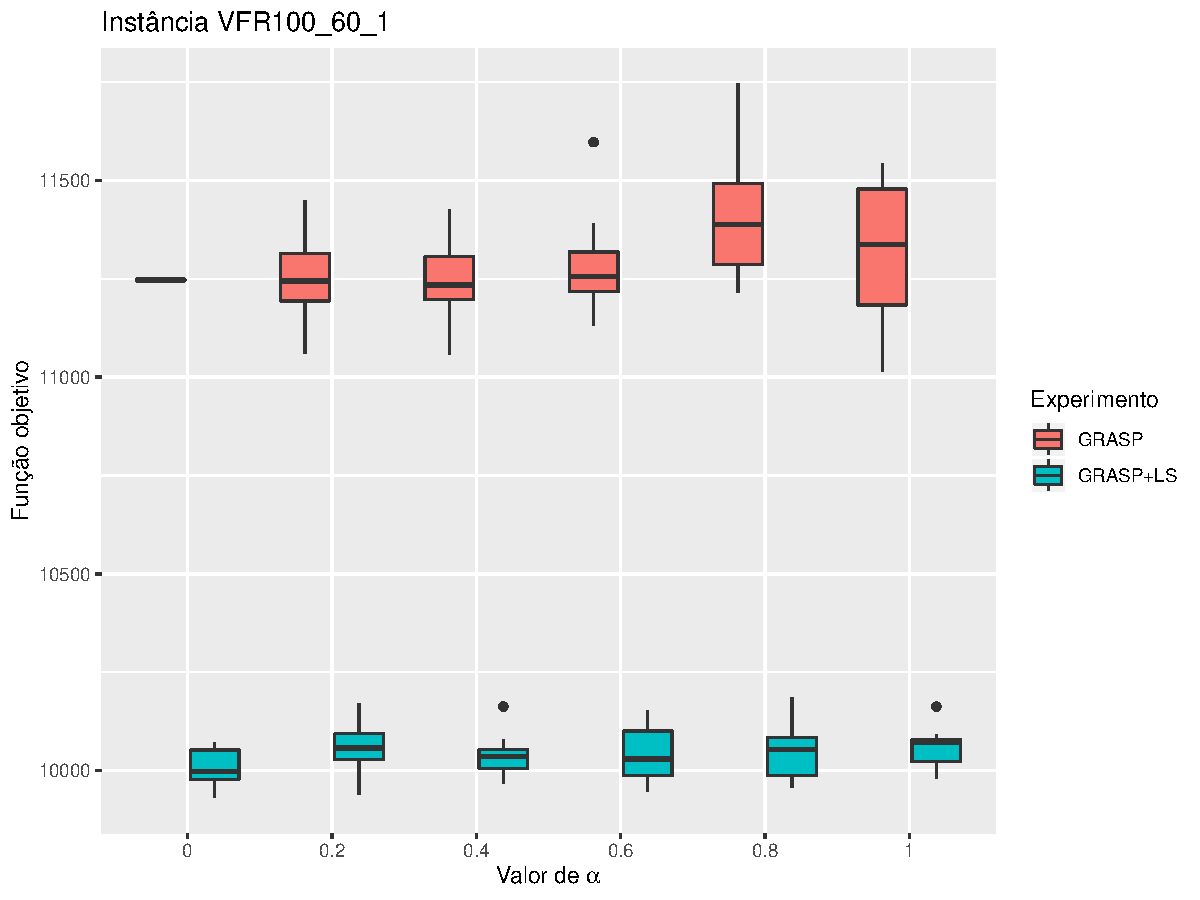
\includegraphics[width=0.48\textwidth]{../resultados/boxplot-VFR100_60_1.pdf}
         }
      }
      \only<4>{
         \subfloat{
            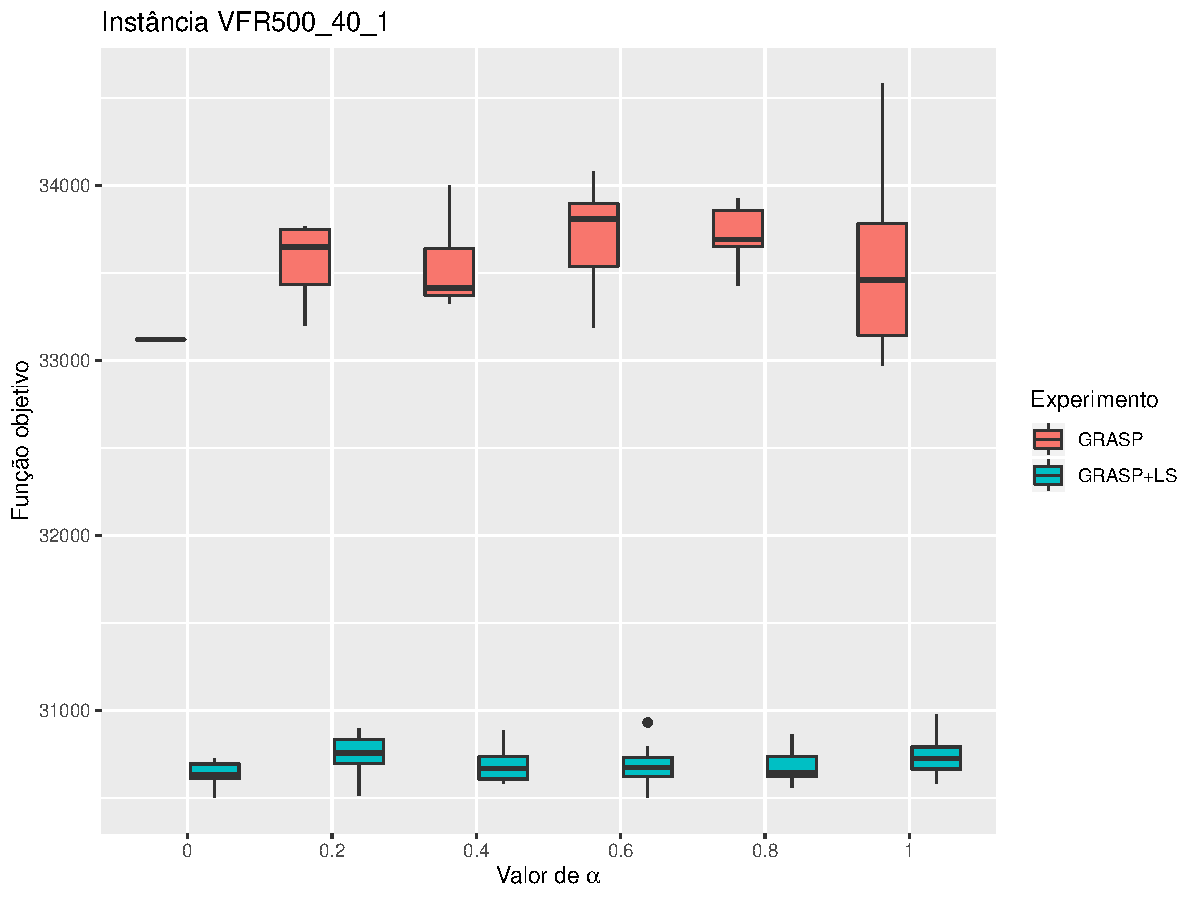
\includegraphics[width=0.48\textwidth]{../resultados/boxplot-VFR500_40_1.pdf}
         }
         \subfloat{
            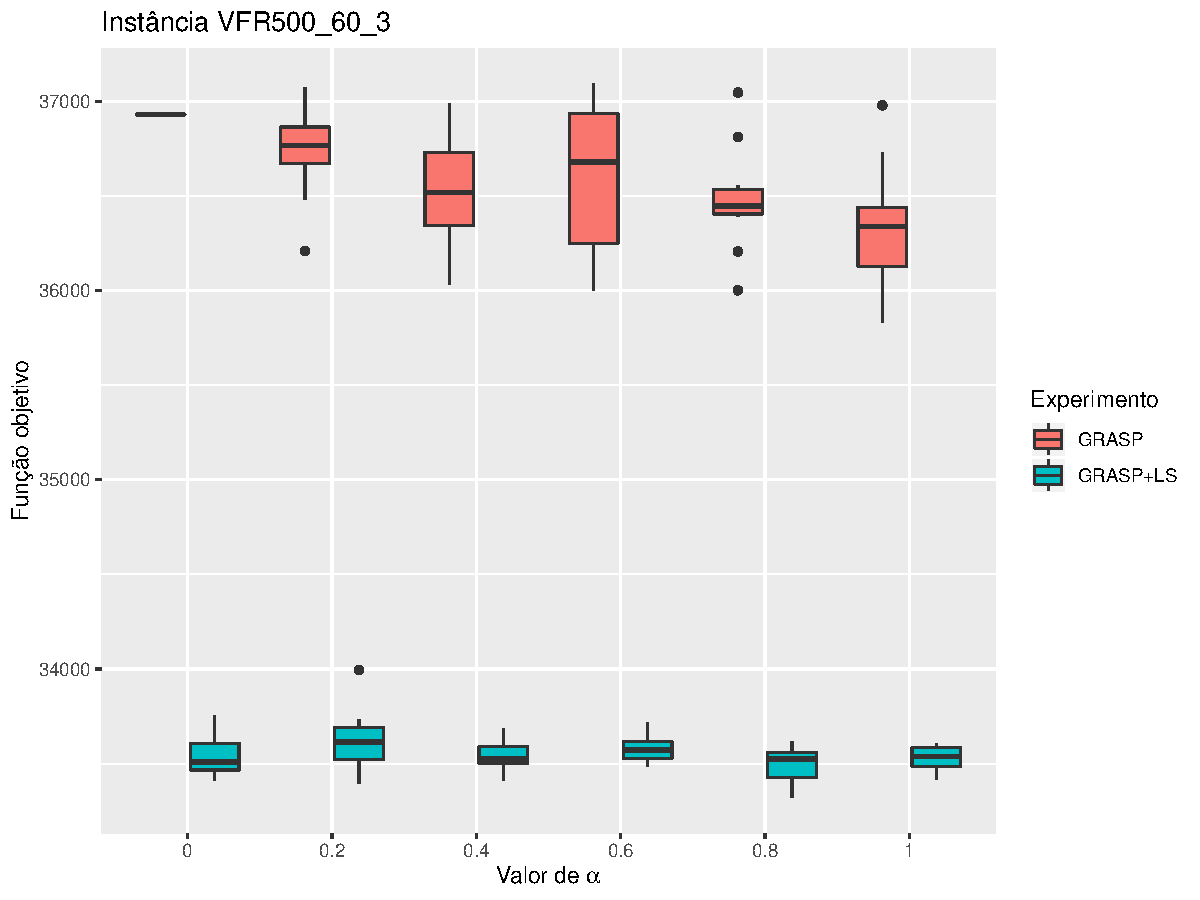
\includegraphics[width=0.48\textwidth]{../resultados/boxplot-VFR500_60_3.pdf}
         }\\
      }
      \only<5>{
         \subfloat{
            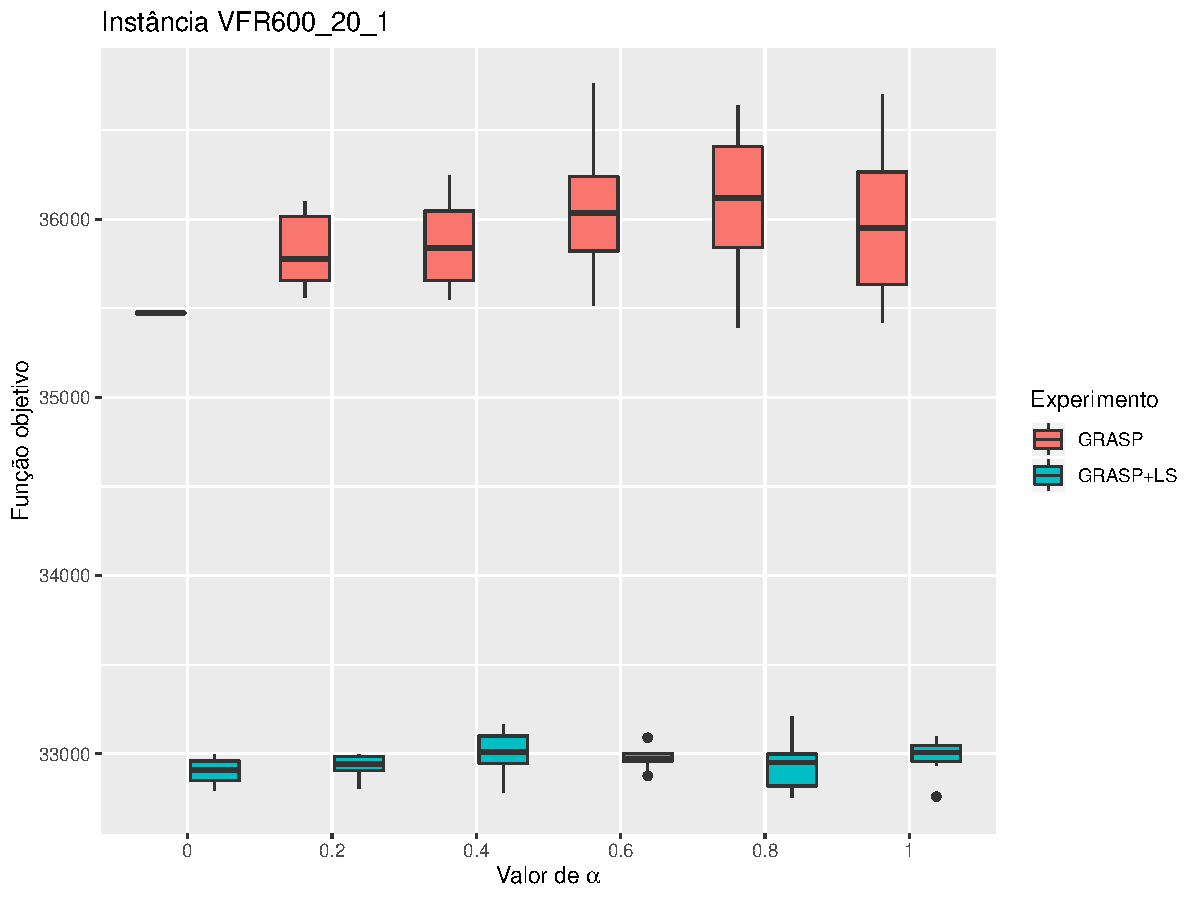
\includegraphics[width=0.48\textwidth]{../resultados/boxplot-VFR600_20_1.pdf}
         }
         \subfloat{
            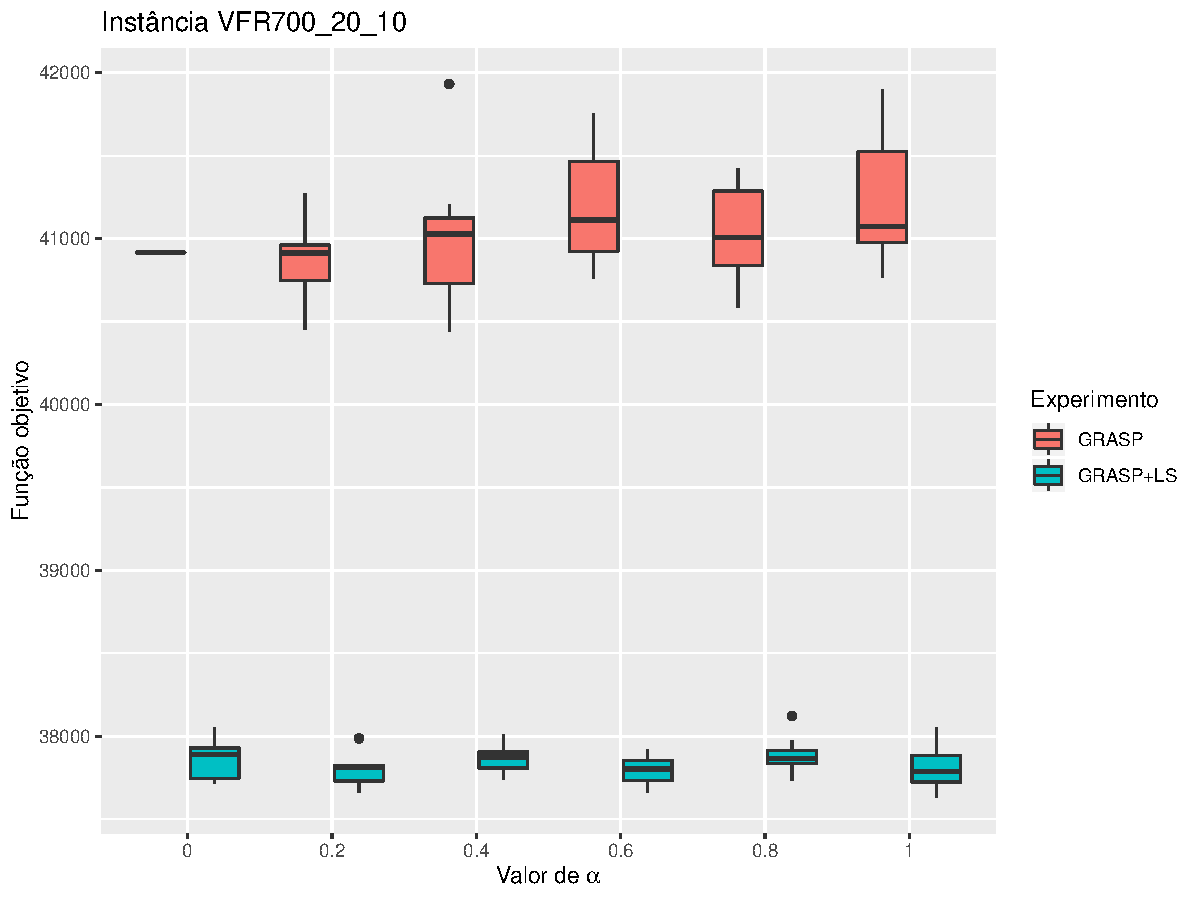
\includegraphics[width=0.48\textwidth]{../resultados/boxplot-VFR700_20_10.pdf}
         }
      }
      \caption{Boxplot relacionando valor médio da função objetivo para as diversas 
         instâncias de testes, com vários valores \bm{$\alpha$} e 10 replicações
         por caso de teste.}
   \end{figure}

\end{frame}

\section{Conclusões}

\begin{frame}
   \frametitle{Observações finais}

   \textbf{PFSP é um problema relevante}
   \begin{itemize}
      \item Abordagem exata é ineficiente
      \item GRASP obtém soluções iniciais rapidamente
      \item Randomização pouco efetiva
      \item Busca Local fez diferença
      \item Heurística foi eficaz e eficiente
   \end{itemize}

   \medskip
   \textbf{Trabalhos futuros}
   \begin{itemize}
      \item Cálculo mais eficiente de custo da vizinhança com \texttt{Swap2LS}
      \item Calibração dos parâmetros
   \end{itemize}

\end{frame}

\section*{Bibliography}

\begin{frame}[allowframebreaks]
  \frametitle{Referências}
  \footnotesize
  \bibliographystyle{plainnat}
  \bibliography{bibliography}
\end{frame}

\section*{}

\begin{frame}[plain]
  \begin{center}
      \LARGE \textbf{Obrigado!} \normalsize \\[24pt]
      Alberto F. K. Neto\\
      \footnotesize
      \smallskip
      \color{InfGray}
      Institute of Informatics (II)\\
      Federal University of Rio Grande do Sul (UFRGS)\\
      \texttt{afkneto@inf.ufrgs.br}\\[8pt]
      
\includegraphics[width=70pt]{inf-logo-white}
  \end{center}
\end{frame}

\end{document}



